%! TeX program = xelatex
\documentclass[12pt, a4paper]{article}
\usepackage{geometry, tikz, float, pgfplots, xcolor, titlesec, amsmath, url, hanging, siunitx, graphicx, sectsty}
\usepackage[utf8]{inputenc}
\usepackage[skip=3pt]{parskip}
\usepackage[none]{hyphenat}
\usepackage[no-math]{fontspec}   % only changes normal font
% Tells LaTeX the images are kept in the "images" folder under the main directory
\graphicspath{ {./assets/} }
\pgfplotsset{compat=1.18, width=10cm}
% Spacing of sections: 0pt on the left, 18pt above, and 12pt below
\titlespacing\section{0pt}{18pt}{12pt}
% font size 12 for the sections
\sectionfont{\fontsize{12}{15}\selectfont}

% Setting font
\setromanfont{Arial}

% Setting strict margins
\sloppy

\begin{document}

\begin{center}

% Extra space at the top of the document
\noindent \\[10pt]
\color{black}

\thispagestyle{empty} % No page number for this page

\Large{\textbf{Properties of Gamma Radiation}} \\[30pt]
\normalsize \textit{Jack Greenberg, Jacob Fairham}\\[5pt]
\textit{11017146,  11074241}\\[20pt]
Department of Physics and Astronomy \\[5pt]
The University of Manchester \\[20pt]
First Year Laboratory Report 2 \\[20pt]
January 2023 \\[25pt]

\end{center}

\textbf{Abstract}\\[12pt]
This expirement aimed to analyze the spectra created using gamma ray spectroscopy using thallium-activated sodium iodide scintillation detectors with radioactive isotopes such as $^{22}$Na, $^{60}$Co, and $^{137}$Cs. The peaks of the $^{22}$Na spectrum were then used to calculate the strength of the sodium source and the relative efficiencies of the detector at the different photopeak energies. Finally, different materials were used between the isotopes and the detector to measure the relation between gamma ray detections and the thickness of the barrier between the source and the detector at different energy levels. We found our isotope of $^{22}$Na had a source strength of $11.77\pm1.81$kBq, as compared to its theoretical $15.09$kBq obtained using the initial source strength as well as the half life of the isotope and the amount of time that has passed from the initial source measurement.

\noindent 

\pagebreak

\section{Introduction}
Gamma radiation was first discovered and studied in 1900 by Paul Villard [citation] however the first quantitative experiment was carried out by Rurtherford and Andrade in 1914; This was carried out through gamma-ray spectroscopy with a rock salt crystal and proved their wavelengths were shorter than the previously studied X-ray radiation [citation]. In 1944, gamma-ray spectroscopy began in earnest with Curran and Baker’s development of the scintillation detector [citation] which, to this day, is still the most popular method for detection of gamma rays. This experiment uses the same detection equipment to explore the three ways gamma radiation interacts with matter: Einstein’s photoelectric effect, Compton scattering and pair production. Each of these interactions produces an electron which can then be analysed to find the original energy of the photon and then processed to create a spectrum of detected photon energies. Exploring properties of gamma radiation is important as it is a powerful tool in imagery and detection. These detection techniques have been utilised to identify the presence of different radioactive isotopes which can aid geological mapping, dating of materials and are also notably used medically with many applications including predominantly imaging of inside human bodies.

\section{Experimental Setup}
This experiment uses a thallium-activated sodium iodide scintillation detector to measure the spectrum of photon energies released. This consists of a rock-salt crystal connected to a photomultiplier tube (PMT) when connected to a multi-channel analyser which converts it to data the computer can process. 
The radiation enters the NaI crystal and excites the electrons. The thallium doping of the crystal then ensures the photon released in the ensuing deexcitation is in the visible light spectrum. This is then incident with the photocathode where an electron is liberated through the photoelectric effect. The PMT then amplifies this signal by leading the electron through cups charged with a large potential difference which cause acceleration and therefore the dislodging of more electrons. By the time the signal reaches the anode at the end, the signal has been multiplied ~1,000,000x.
This electrical signal is then sent to the multi-channel analyser which processes it into different channels corresponding to energy levels of photons. To give specific energies, data must be recorded for each source and then used with the known values of photopeak energies [citation] to calibrate each channel to an energy value.

	\begin{figure}[H] \centering
		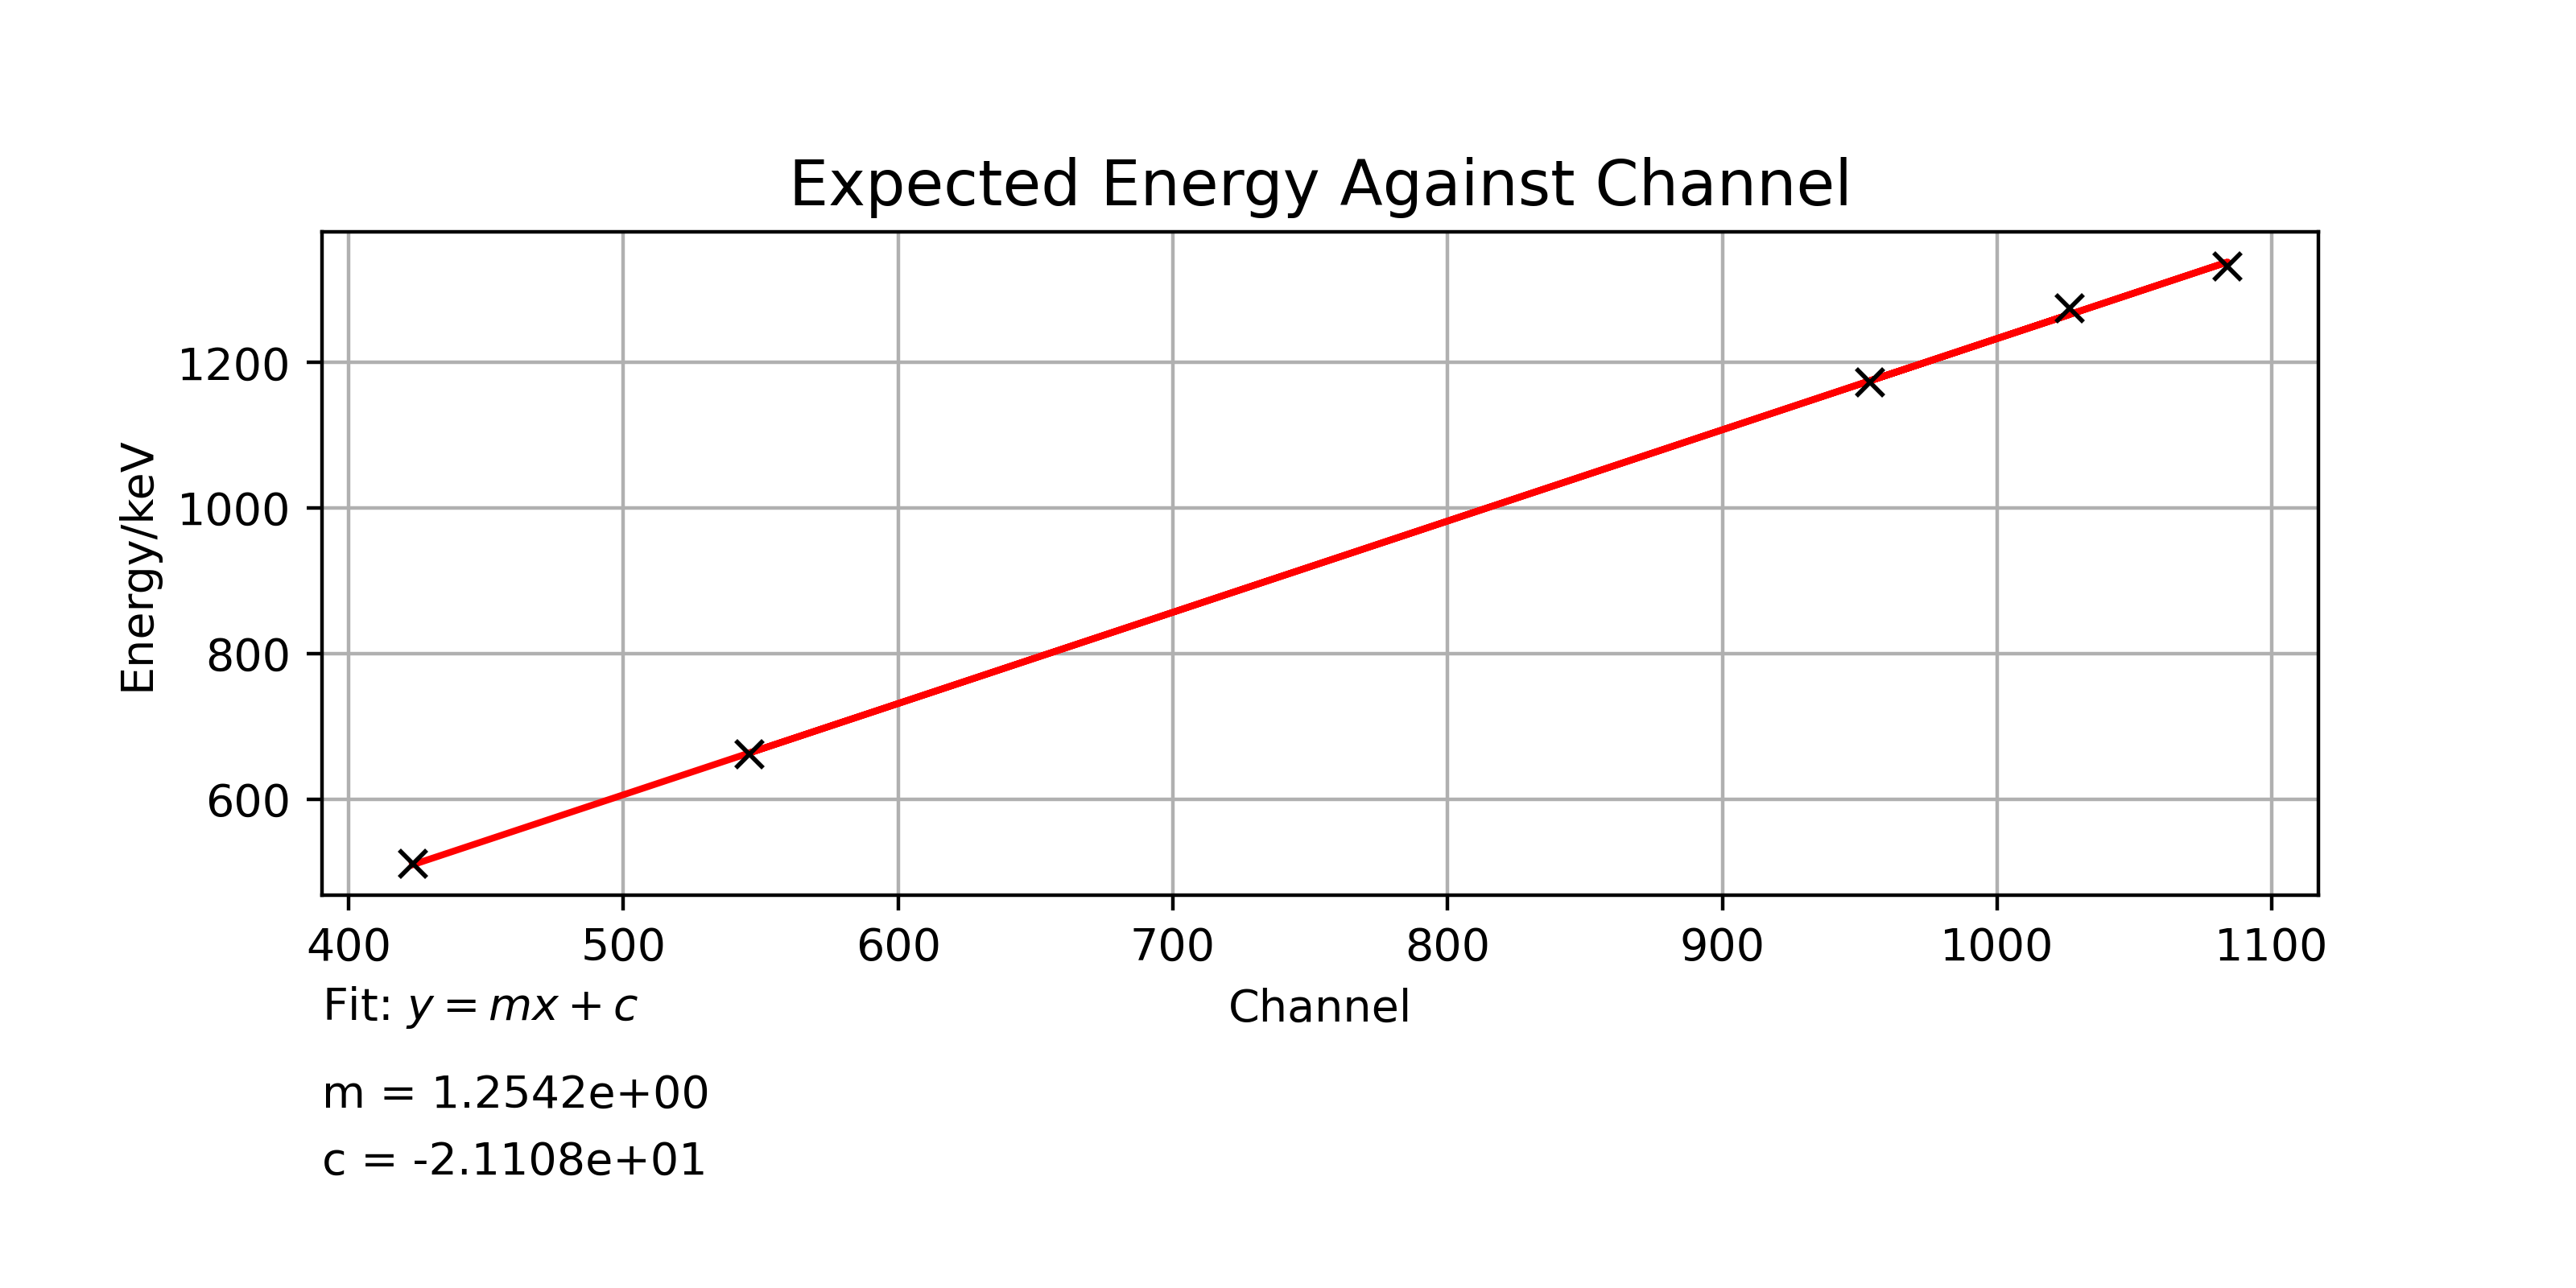
\includegraphics[scale=0.5]{assets/Calibration.png}
		\caption{LSFR plot for conversion from channels to energy}
	\end{figure}

Figure 1 shows the relation between channel and energy to be
\begin{equation}
	(Energy/\unit{\keV}) = 1.25(Channel)+1.66
\end{equation}
which can then be input to the software 'Maestro' which automatically converts all channels to their corresponding energies

\section{Interpreting the Spectra}
The spectra obtained from measuring each source in the open air display four regions of importance. The tall, wide 'photopeaks' correspond to electrons detected through the photoelectric effect, matching the decay patterns of the isotopes. The wide spread before each photopeak represents regions of Compton background radiation, where a photon has hit an electron which is then scattered with energies dependant on the angle of scattering $\theta$
	\begin{equation}
		E_{final} = \frac{E_{initial}}{1+(\frac{E_{initial}}{m_{electron}c^{2}})(1-cos\theta)}
	\end{equation}
gives the final energy of the photon so
	\begin{equation}
	E_{electron} = E_{initial}-E_{final}
	\end{equation}
which has a maximum at $\theta$=$180^{\circ}$ which is where a drop in counts is found known as the 'Compton edge'. Inversely, at the lower energy end of compton scattering the 'backscatter peak' can be found. This is where the scattered photons return to the detector instead of the electrons and then, through the photoelectric effect, cause a low energy electron to be detected.
\begin{figure}[H] \centering
		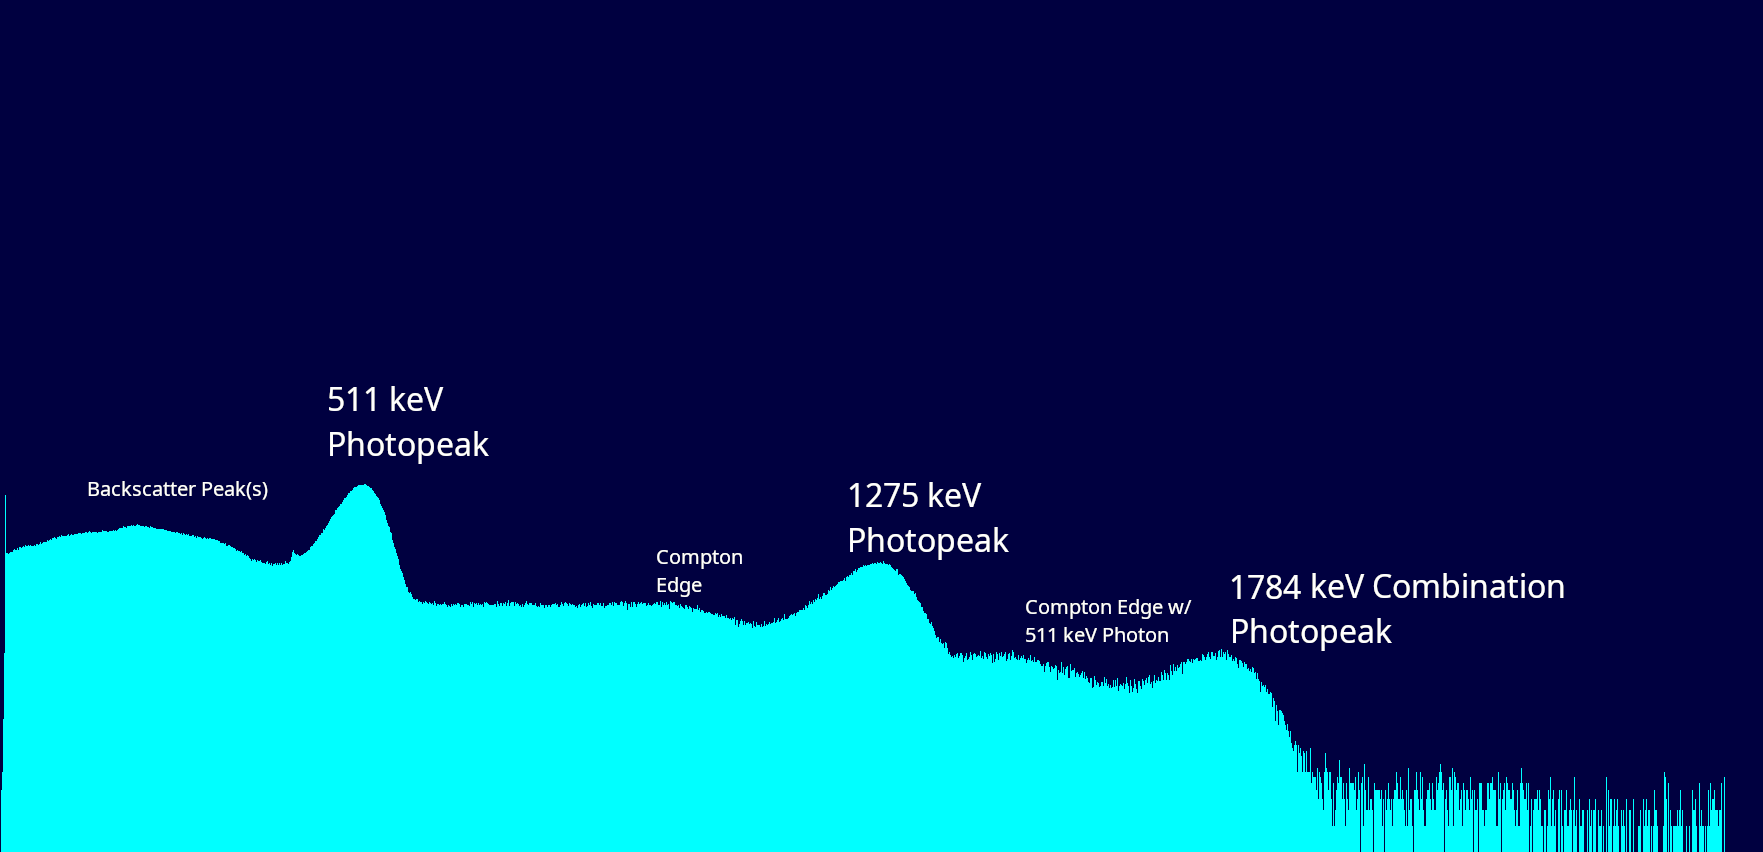
\includegraphics[scale=0.3]{assets/na22_log_annotated.png}
		\caption{Spectrum of Sodium 22 - Log scale counts by energy}
	\end{figure}
The Sodium-22 spectrum also displays a 'sum peak' where the detector registers both the $511\unit{Kev}$ and $1275\unit{Kev}$ photons as one since the delay between the deexcitation from the 1275 line and the positron annihilation reaction is unresolvably small
	\begin{figure}[H] \centering
		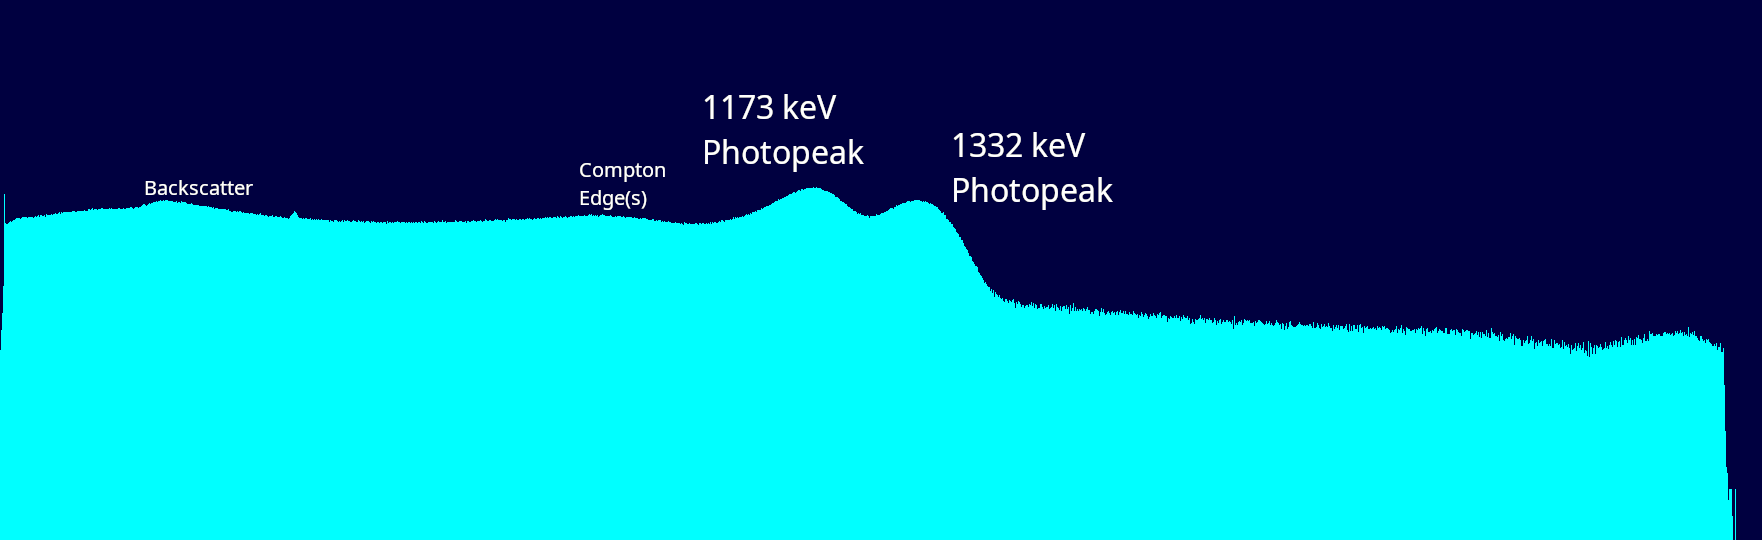
\includegraphics[scale=0.3]{assets/co60_log_annotated.png}
		\caption{Spectrum of Cobalt 60 - Log scale counts by energy}
	\end{figure}
	\begin{figure}[H] \centering
		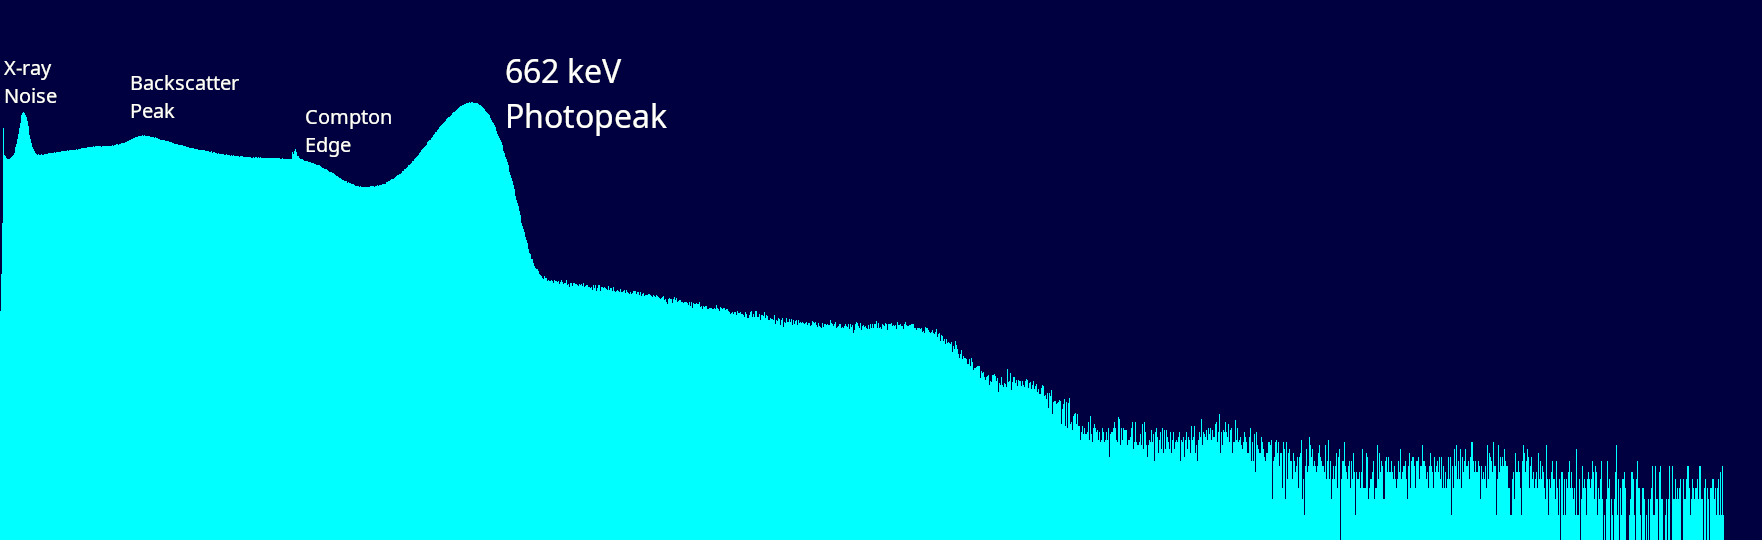
\includegraphics[scale=0.3]{assets/cs137_log_annotated.png}
		\caption{Spectrum of Cesium 137 - Log scale counts by energy}
	\end{figure}
In figure 4, a sharp, low energy peak is seen which corresponds to X-ray radiation originating from the orbital electrons of the source as opposed to the nucleic decay producing higher energy photons.
\section{Source Strength Measurements}
	The decay process for $^{22}$Na involves two $511\unit{\keV}$ photons and one $1275\unit{\keV}$ photon. The detector comprises some fraction of the solid angle $\Omega$. The probability of a detection of a $511\unit{\keV}$ and a $1275\unit{\keV}$ photon is
	\begin{equation}
		P(511\unit{\keV}) = 2\Omega\cdot\epsilon(E=511\unit{\keV})
	\end{equation}
	\begin{equation}
		P(1275\unit{\keV}) = \Omega\cdot\epsilon(E=1275\unit{\keV})
	\end{equation}
	thus the probability of the combination sum peak is
	\begin{equation}
		P(1786\unit{\keV}) = P(511\unit{\keV})\cdot P(1275\unit{\keV}) = 2\Omega^2\cdot\epsilon(E=511\unit{\keV})\epsilon(E=1275\unit{\keV})
	\end{equation}
	the rate of detecton for each of the peaks ($R_E$) is a measurable value and is the source strength ($S$) times the probability of the peak. The following measurements were taken over $6600\unit{\s}$:
	\begin{align}
		R_{511} &= 202.56\pm.60\unit{\becquerel}\\
		R_{1275} &= 45.35\pm.32\unit{\becquerel}\\
		R_{1786} &= 0.78\pm.12\unit{\becquerel}
	\end{align}
	which allows the calculation of the ratio of the efficiencies of the detector at different energies
	\begin{equation}
		\frac{\epsilon(E=511\unit{\keV})}{\epsilon(E=1275\unit{\keV})} = \frac{R_{511}}{2R_{1275}} = 2.23\pm.02
	\end{equation}
	and the calculation of the source strength by
	\begin{equation}
		S = \frac{R_{511}\cdot R_{1275}}{R_{1786}} = 11.8\pm1.8\unit{\kilo\becquerel}
	\end{equation}
	where the errors on the measured values arise from subtracting background noise from the gross area in the spectrum and the errors on the calculated values arise from standard error propogation.

\section{Gamma Ray Absorption}
	It can be shown through a simple differential calculation that
	\begin{equation}
		I = I_0 e^{\frac{x}{\tau}}
	\end{equation}
	where $\tau$ is a function of the energy/wavelength of the photon. Therefore, by categorizing the data by photopeak energy and plotting the rate of detection by the thickness of the material for each separate material, we can calculate different values of $\tau$ and relate the absorption of the materials to each other. The predominant cause of error was the time window that measurements were taken in. Ideally, since cobalt has a considerably lower count rate than the other sources, it would have been measured for an appropriately longer time.
	\begin{figure}[H] \centering
		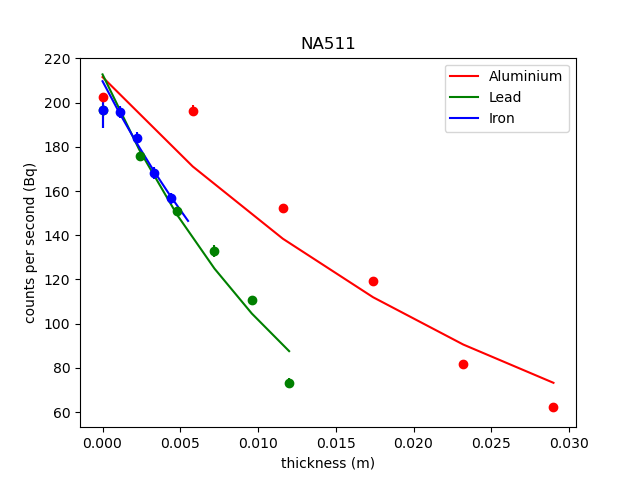
\includegraphics[scale=0.4]{assets/NA511.png}
		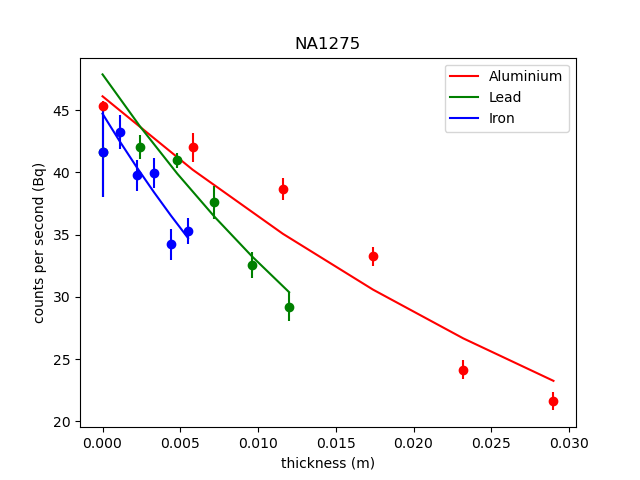
\includegraphics[scale=0.4]{assets/NA1275.png}
		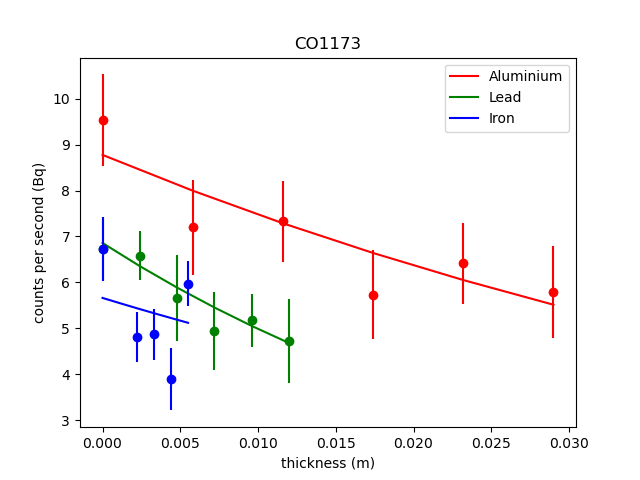
\includegraphics[scale=0.4]{assets/CO1173.png}
		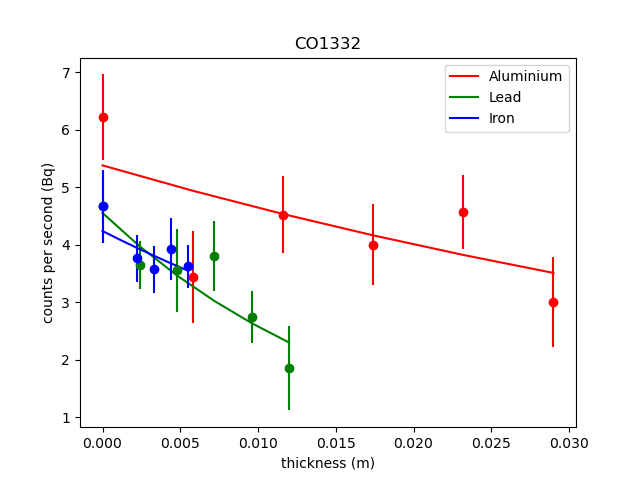
\includegraphics[scale=0.4]{assets/CO1332.png}
		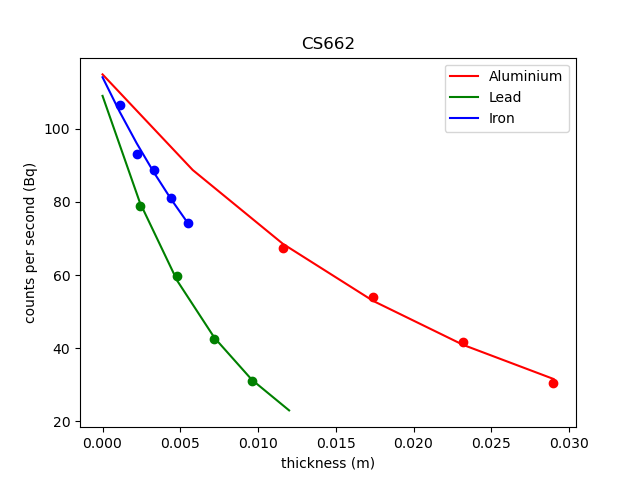
\includegraphics[scale=0.4]{assets/CS662.png}
		\caption{Counts per second measured for different thicknesses of different materials - each graph is of a different photopeak. Fit data shown below}
	\end{figure}

	\small{
		\begin{center}
			\begin{tabular}{ ||c|c|c|c|c|c|| }
				$\tau$ & NA511 & NA1275 & CS662 & CO1173 & CO1332\\ 
				Aluminium & $0.027\pm0.002$ & $0.042\pm0.005$ & $0.022\pm0.003$ & $0.062\pm0.043$ & $0.068\pm0.047$\\
				Iron & $0.015\pm0.007$ & $0.022\pm0.015$ & $0.013\pm0.002$ & $0.055\pm0.125$ & $0.031\pm0.039$\\
				Lead & $0.014\pm0.002$ & $0.026\pm0.009$ & $0.008\pm0.001$ & $0.031\pm0.021$ & $0.018\pm0.006$\\
				$\chi^2$ & & & & & \\ 
				Aluminium & $13.66$ & $4.47$ & $0.39$ & $0.59$ & $3.03$\\
				Iron & $0.14$ & $0.49$ & $0.50$ & $4.14$ & $0.65$\\
				Lead & $3.24$ & $0.80$ & $0.24$ & $0.23$ & $2.34$\\
			\end{tabular}
		\end{center}
	}

\section{Data}
	Raw data is availible electronically[2].

\section{Analysis}
	analysis

\section{Conclusion}
	conclusion

\section*{References}

	\begin{hangparas}{.25in}{1}
		[1] Ocaya, Richard. (2006). An experiment to profile the voltage, current and temperature behaviour of a P-N diode. European Journal of Physics. 27. 625. 10.1088/0143-0807/27/3/015.
		
		[2] Daussy, C. et al. "Direct Determination of the Boltzmann Constant by an Optical Method". Phys. Rev. Lett. 98. (2007): 250801.
	\end{hangparas}

\end{document}
